If you haven't downloaded and unzipped \href{https://libaoj.in/courses/2021f/MATH3341/zip/Math.3341.zip}{\texttt{Math.3341.zip}}. Download and unzip it under \verb|H:| (H Drive if you are working on the Remote Lab). Change the current working directory by typing \verb|cd H:\Math.3341\Math.3341.Lab.06| in the Command Window, and type \verb|edit lab_06_script| in the Command Window to edit \verb|lab_06_script.m|.

%---------------------------------------------
\section{Solve a System with LU Decomposition}
%---------------------------------------------
\label{sec:lu}
\begin{enumerate}[(a)]
\item Define matrix \verb|A| and vector \verb|b| as \eqref{eq:ls}.
  \begin{equation}
  \label{eq:ls}
  \underbrace{
  \begin{bmatrix}
    7 & -26 &  45 & -47 \\
    1 &   2 &   3 &   4 \\
    2 & -11 & -12 & -13 \\
    4 & -17 &  30 &  35 \\
  \end{bmatrix}}_{A}
  \underbrace{
  \begin{bmatrix}
    x_1 \\
    x_2 \\
    x_3 \\
    x_4 \\
  \end{bmatrix}}_{\mathbf{x}}
  =
  \underbrace{
  \begin{bmatrix}
     -98 \\
      30 \\
    -108 \\
     200 \\
  \end{bmatrix}}_{\mathbf{b}}
  \end{equation}
\item Calculate the LU decomposition \verb|L|, \verb|U| of the matrix \verb|A|.
\item \label{enu:lz} Solve the following system \eqref{eq:lz} and store the solution to \verb|z|.
  \begin{equation}
  \label{eq:lz}
  L \mathbf{z} = \mathbf{b}.
  \end{equation}
\item \label{enu:ux} Then solve the following system \eqref{eq:ux} and store the solution to \verb|x|.
    \begin{equation}
    \label{eq:ux}
    U \mathbf{x} = \mathbf{z}.
    \end{equation}
\item Check your solution by calculating the norm of the residual $\|A\mathbf{x} - \mathbf{b}\|_2$ and store the result to \verb|res|.
\end{enumerate}
%---------------------------------------------
\section{Varying the Vector $\mathbf{b}$}
%---------------------------------------------
Suppose we want to solve the system for each integer value of $m$ in between $m = 0$ and $m = 20$. This time use the LU decomposition of the system matrix; perform the decomposition only once and use the lower and upper triangular factors repeatedly to find each successive solution. Then generate a table (Table \ref{tab:solution}) and a plot (Figure \ref{fig:solution}) of the solution versus the integer $m$.
\begin{equation}
  \label{eq:sys}
  \begin{cases}
    3 x + y + z = m \\
    x - 5 y + 2 z = 5 \\
    2 x + y + 5 z = 10 \\
  \end{cases}
\end{equation}
To do this you'll follow the steps below:
\begin{enumerate}[(a)]
\item Define coefficient matrix \verb|A| given in \eqref{eq:sys}, and get the LU decomposition \verb|L|, \verb|U| of the matrix \verb|A|.
\item Define a vector \verb|m| which ranges from $0$ to $20$ with step size $1$.
\item Then create a for-loop, of which the loop iterator \verb|i| starts from \verb|1| to \verb|length(m)|. In the body of the loop, define a column vector \verb|b| as the right-hand side of \eqref{eq:sys}, where $m$ should be the \verb|i|th component of \verb|m|. Then repeat \eqref{enu:lz} and \eqref{enu:ux} in Part \ref{sec:lu}. Store the solution \verb|x| to the \verb|i|th row of \verb|X|.
\item Format the output of \verb|m| and \verb|X| to a file called \verb|solution.tex| as you did in Part 3 of Lab 05:
  \begin{enumerate}[(i)]
    \item Use \verb|fprintf| to print out the setup for the \emph{table} and \emph{tabular} environments. The first column of the table is centered while the rest three columns are right-justified in \LaTeX{}.
    \item Between \verb|\toprule| and \verb|\midrule|, use \verb|fprintf| to print out the heading of the table. The column widths are $4, 11, 11, 11$, respectively.
    \item Between \verb|\midrule| and \verb|\bottomrule|, use a for-loop to print each row of the table. Note that the $i$th row of the table consists of the \verb|i|th component of \verb|m| and the \verb|i|th row of matrix \verb|X|. The column widths are $2, 9, 9, 9$, respectively. For floating point numbers, output 6 digits after the decimal point.
    \item Call \verb|type('solution.tex')| to print the content of \verb|solution.tex|.
  \end{enumerate}
\item Plot the solution versus $m$ using a for-loop as you did in Part 4 of Lab 05:
  \begin{enumerate}[(i)]
    \item Get the size of \verb|X| and assign it to \verb|XSize|. Define a cell array \verb|styles|, of which the entries are dashed line with hexagram, dotted line with pentagram, solid line with diamond.
    \item The use a for-loop to plot each column of \verb|X| versus \verb|m| in the same figure window with the above styles.
    \item Add labels, title, grid, legend as shown in Figure \ref{fig:solution}.
    \item Save the plot to a file named \verb|lab_06_plot.pdf|.
  \end{enumerate}
\end{enumerate}
%---------------------------------------------
Type \verb|diary('lab_06_output.txt')| in the Command Window, run the script file \verb|lab_06_script.m|, and type \verb|diary off| in the Command Window. Upload \verb|lab_06_output.txt|, \verb|lab_06_script.m|, \verb|solution.tex|, and \verb|lab_06_plot.pdf| to the folder \verb|src| on Overleaf.

On Overleaf, open \verb|body.tex| under the folder \verb|LaTeX|. In the last section of the report, you will reproduce Section \ref{sec:bol} using \LaTeX{}. You may find the following helpful:

\begin{itemize}
  \item You may use enviroments such as  \verb|equation|, \verb|cases|, \verb|figure|, and \verb|table|.
  \item You may use \verb|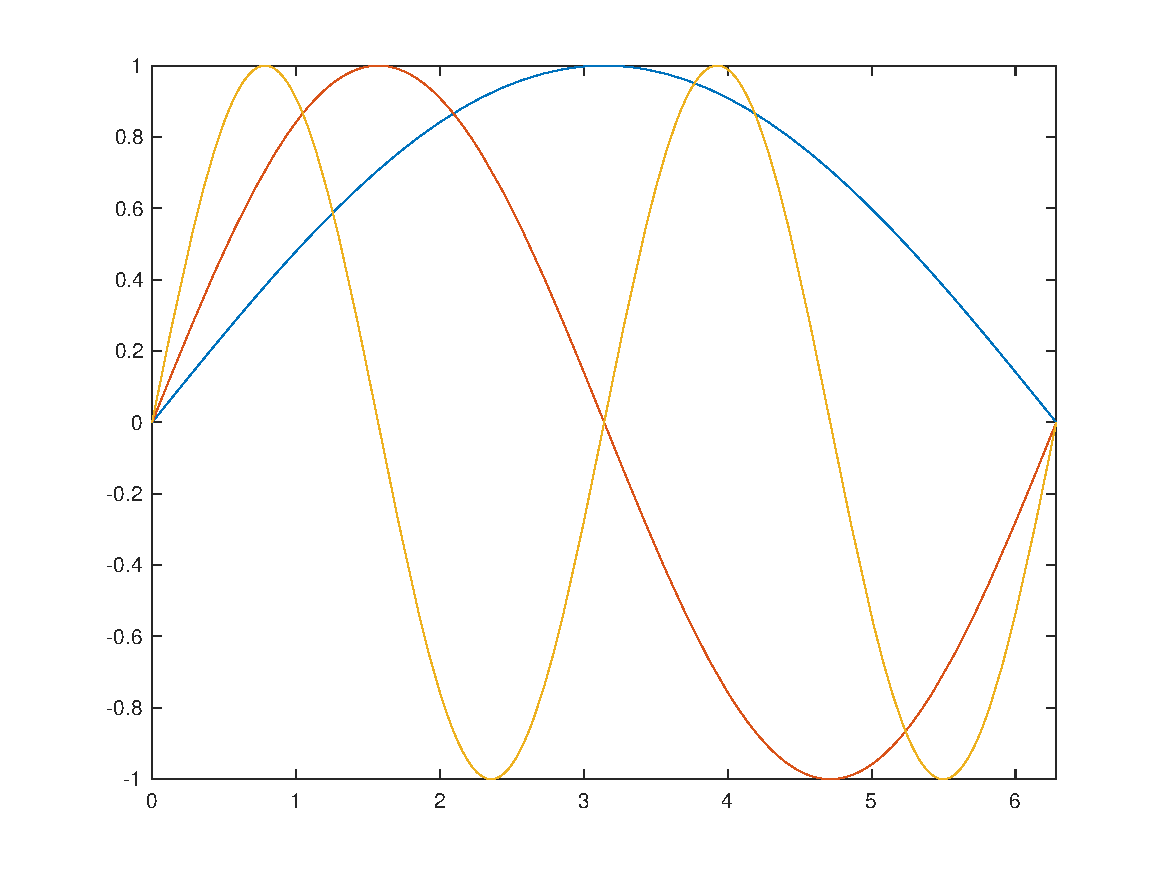
\includegraphics[width=amount unit]{/path/to/figure.pdf}| to specify the width of a figure. In our case, the width of the figure is \verb|0.85\textwidth|.
  \item You may use \verb|\ref{labelName}| to refer to figures, tables; use \verb|\eqref{labelName}| to refer to equations.
  \item For special symbols, you may look them up in \href{https://libaoj.in/files/LaTeX.Mathematical.Symbols.pdf}{\LaTeX{}.Mathematics.Symbols.pdf}.
  \item You may use \verb|%
% main.tex
%
% Copyright © 2019 Libao Jin <jinlibao@outlook.com>
% Distributed under terms of the MIT license.
%

\documentclass[11pt,oneside,letter,twoside,usename,dvipsnames,svgnames,table]{article}

% Load packages
\usepackage{
  afterpage,amsfonts,amsmath,amssymb,amsthm,appendix,array,booktabs,breqn,
  caption,color,enumerate,enumitem,fancyhdr,float,fontspec,geometry,graphicx,grffile,
  hyperref,hyphenat,ifthen,imakeidx,indentfirst,lastpage,lipsum,listings,
  longtable,makeidx,mathtools,multicol,subcaption,tikz,tikzscale,titlesec,
  titling,verbatim,xcolor,xltxtra,xunicode
}

\title{MATH 3340 - Scientific Computing Homework 8}
\author{Libao Jin}

\makeatletter
\let\Author\@author
\let\Title\@title
\makeatother
% ------------------- define \Xint ----------------
\def\Xint#1{\mathchoice
  {\XXint\displaystyle\textstyle{#1}}%
  {\XXint\textstyle\scriptstyle{#1}}%
  {\XXint\scriptstyle\scriptscriptstyle{#1}}%
  {\XXint\scriptscriptstyle\scriptscriptstyle{#1}}%
\!\int}
\def\XXint#1#2#3{{\setbox0=\hbox{$#1{#2#3}{\int}$ }
\vcenter{\hbox{$#2#3$ }}\kern-.6\wd0}}
\def\ddashint{\Xint=}
\def\dashint{\Xint-}
% ------------------- setlength -------------------
\setlength{\parindent}{0pt}
\setlength{\parskip}{5pt}
% ------------------- algorithm2e -----------------
\usepackage[ruled]{algorithm2e}
% ------------------- amsthms ---------------------
\theoremstyle{definition}
\newtheorem{definition}{Definition}[section]
\newtheorem{lemma}{Lemma}[section]
\newtheorem{corollary}{Corollary}[section]
\newtheorem{remark}{Remark}[section]
\newtheorem{claim}{Claim}[section]
\newtheorem{theorem}{Theorem}[section]
\newtheorem{example}{Example}[section]
\newtheorem{exercise}{Exercise}[section]
\newtheorem{proposition}{Proposition}[section]
\newtheorem{proc}{Procedure}[section]
\numberwithin{equation}{section}
% ------------------- define macros ---------------
\newcommand{\tightlist}{}
\newcommand{\semester}{\ifthenelse{\month<9}{\ifthenelse{\month<5}{Spring}{Summer}}{Fall} \the\year}
\newcommand{\AxisRotator}[1][rotate=0]{%
  \tikz [x=0.25cm,y=0.60cm,line width=.2ex,-stealth,#1] \draw (0,0) arc (-150:150:1 and 1);%
}
% \newcommand{\problem}{0}
\newcommand{\sol}{0}
\newcommand{\homework}{0}
\ifdefined\problem
  \newenvironment{solution}{\comment}{\endcomment}
\else
  \newenvironment{solution}{\begin{proof}[{\rm\bf Solution}]}{\end{proof}}
  \newcommand{\sectionbreak}{\clearpage}
\fi
% ------------------- titlesec --------------------
\ifdefined\homework
  \titleformat{\section}[runin]{\bf}{}{0em}{}[.]
\fi
%\titleformat{\section}{\scshape\Large}{\thesection}{1em}{}
%\titleformat{\subsection}{\scshape\large}{\thesubsection}{1em}{}
%\titleformat{\subsubsection}{\large}{\thesubsubsection}{1em}{}
%\renewcommand{\thesection}{\Roman{section}}
% ------------------- caption ---------------------
\captionsetup{width=0.95\textwidth}
% ------------------- enumitem --------------------
\setlist{noitemsep}
% \setenumerate{label=(\alph*)}
% ------------------- fontspec --------------------
% \defaultfontfeatures{Mapping=tex-text,Scale=MatchLowercase,Numbers=OldStyle}
% \setromanfont{Palatino}
% \setsansfont{Helvetica}
\setmonofont[Scale=MatchLowercase]{Monaco}
% ------------------- geometry --------------------
\geometry{
  margin = 1in
}
% ------------------- hyperref --------------------
\hypersetup{
  %--------------- pdfinfo ------------------
  pdftitle  = {\Title},
  pdfauthor = {\Author},
  pdfsubject= {\Title},
  pdfkeywords={},
  %--------------- links --------------------
  colorlinks= {true},
  linkcolor = {red},
  citecolor = {cyan},
  bookmarks = {false},
  bookmarksnumbered = {true},
  %--------------- pagemode -----------------
  pdffitwindow={true},
  pdftoolbar= {false},
  pdfmenubar= {false},
  pdfpagelayout = {OneColumn},
  pdfstartview = {FitH},
  pdfpagemode = {UseNone},
  %pdfnonfullscreenpagemode = {UseNone}
}
%------------------- fancyhdr ---------------------
\fancypagestyle{exercise-style}{
  \fancyhf{}
  \fancyhead[LO,RE]{\footnotesize \semester}
  \fancyhead[CO,CE]{\footnotesize \Title}
  \fancyhead[LE,RO]{\footnotesize\thepage\ of \pageref*{LastPage}}
  \pagenumbering{arabic}
}
\fancypagestyle{report-style}{
  \fancyhf{}
  \fancyhead[LO,RE]{\footnotesize \Author}
  \fancyhead[CO,CE]{\footnotesize \Title}
  \fancyhead[LE,RO]{\footnotesize\thepage\ of \pageref*{LastPage}}
  \pagenumbering{arabic}
}
\renewcommand{\sectionmark}[1]{\markboth{#1}{}}
\renewcommand{\subsectionmark}[1]{\markright{\thesubsection \ #1}}
\pagestyle{report-style}
% ------------------- maketitle -------------------
\makeatletter
\def\@maketitle{%
  \begin{center}%
    \let \footnote \thanks
    %{\bfseries\huge \course\ --- \semester \par \vskip .5em {\LARGE \@title}}
    {\LARGE \@title \par}
    {\vskip 1.5em \large \@author}
    {\vskip .5em \large \@date}
  \end{center}
\par \vskip .5em}
\makeatother
% ------------------- table alignment -------------
\newcolumntype{L}[1]{>{\raggedright\arraybackslash}p{#1}}
\newcolumntype{C}[1]{>{\centering\arraybackslash}p{#1}}
\newcolumntype{R}[1]{>{\raggedleft\arraybackslash}p{#1}}
% \allowdisplaybreaks
% ------------------ lstlisting ------------------
\lstset{
  basicstyle={\ttfamily\footnotesize},
  breaklines=true,
  keywordstyle=\color{Red},
  otherkeywords={},
  morekeywords={},
  identifierstyle=\color{darkgray},
  stringstyle=\color{LightCoral},
  commentstyle=\color{gray},
  showstringspaces=false,
  numberstyle={\footnotesize \color{Black}},
  numbersep=9pt,
  numbers=left,
  emph={int,char,double,float,unsigned,auto},
  emphstyle={\color{Cerulean}},
  frame=single,
  backgroundcolor=\color{White},
  tabsize=4,
  language={},
}

% Define language diff (using git diff highlighting)
\newcommand{\lstbg}[3][0pt]{{\fboxsep#1\colorbox{#2}{\strut #3}}}
\lstdefinelanguage{diff}{
  basicstyle={\ttfamily\small},
  breaklines=true,
  morecomment=[f][\lstbg{red!20}]-,
  morecomment=[f][\lstbg{green!20}]+,
  morecomment=[f][\color{blue}]{@@},
}

% Define language Golang
\lstdefinelanguage{Golang}%
{morekeywords=[1]{package,import,func,type,struct,return,defer,panic,%
  recover,select,var,const,iota,},%
  morekeywords=[2]{string,uint,uint8,uint16,uint32,uint64,int,int8,int16,%
    int32,int64,bool,float32,float64,complex64,complex128,byte,rune,uintptr,%
  error,interface},%
  morekeywords=[3]{map,slice,make,new,nil,len,cap,copy,close,true,false,%
  delete,append,real,imag,complex,chan,},%
  morekeywords=[4]{for,break,continue,range,goto,switch,case,fallthrough,if,%
  else,default,},%
  morekeywords=[5]{Println,Printf,Error,Print,},%
  sensitive=true,%
  morecomment=[l]{//},%
  morecomment=[s]{/*}{*/},%
  morestring=[b]',%
  morestring=[b]",%
  morestring=[s]{`}{`},%
}

% Define various styles for different lanuages
\lstdefinestyle{Makefile}{
  basicstyle=\ttfamily,
  breaklines=true,
  keywordstyle=\color{Red},
  otherkeywords={},
  morekeywords={},
  identifierstyle=\color{darkgray},
  stringstyle=\color{darkgray},
  commentstyle=\color{gray},
  showstringspaces=false,
  numberstyle={\footnotesize \color{Black}},
  numbersep=9pt,
  numbers=left,
  emph={int,char,double,float,unsigned,auto},
  emphstyle={\color{Cerulean}},
  frame=single,
  backgroundcolor=\color{White},
  tabsize=4,
  language=make,
}

\lstdefinestyle{MATLAB}{
  basicstyle={\ttfamily\small},
  breaklines=true,
  keywordstyle=\color{Red},
  otherkeywords={},
  alsoletter={...},
  morekeywords={break,case,catch,continue,elseif,else,end,for,function,global,
    if,otherwise,persistent,return,switch,try,while,methods,properties,
  events,classdef,...},
  comment=[l]\%,                              % comments
  morecomment=[l]...,                         % comments
  morecomment=[s]{\%\{}{\%\}},                % block comments
  morestring=[m]
  identifierstyle=\color{darkgray},
  stringstyle=\color{LightCoral},
  commentstyle=\color{gray},
  showstringspaces=false,
  numberstyle={\footnotesize \color{Black}},
  numbersep=9pt,
  numbers=left,
  emph={int,char,double,float,unsigned,auto},
  emphstyle={\color{Cerulean}},
  frame=single,
  backgroundcolor=\color{White},
  tabsize=4,
  language=MATLAB,
}

\lstdefinestyle{C++}{
  basicstyle=\ttfamily,
  breaklines=true,
  keywordstyle=\color{Red},
  otherkeywords={memset},
  morekeywords={>,<,.,;,-,!,=,~},
  identifierstyle=\color{darkgray},
  stringstyle=\color{LightCoral},
  commentstyle=\color{gray},
  showstringspaces=false,
  numberstyle={\footnotesize \color{Black}},
  numbersep=9pt,
  numbers=left,
  emph={bool,int,char,double,float,unsigned,auto,string,pair,unordered_set,vector},
  emphstyle={\color{Cerulean}},
  frame=single,
  backgroundcolor=\color{White},
  tabsize=4,
  language=C++,
}

\lstdefinestyle{Plain}{
  basicstyle={\ttfamily\footnotesize},
  breaklines=true,
  keywordstyle=\color{Red},
  otherkeywords={},
  morekeywords={},
  identifierstyle=\color{darkgray},
  stringstyle=\color{LightCoral},
  commentstyle=\color{gray},
  showstringspaces=false,
  numberstyle={\footnotesize \color{Black}},
  numbersep=9pt,
  numbers=left,
  emph={int,char,double,float,unsigned,auto},
  emphstyle={\color{Cerulean}},
  frame=single,
  backgroundcolor=\color{White},
  tabsize=4,
  language={},
}

\lstdefinestyle{TeX}{
  basicstyle={\ttfamily\footnotesize},
  breaklines=true,
  keywordstyle=\color{Red},
  otherkeywords={},
  morekeywords={},
  identifierstyle=\color{darkgray},
  stringstyle=\color{LightCoral},
  commentstyle=\color{gray},
  showstringspaces=false,
  numberstyle={\footnotesize \color{Black}},
  numbersep=9pt,
  numbers=left,
  emph={int,char,double,float,unsigned,auto},
  emphstyle={\color{Cerulean}},
  frame=single,
  backgroundcolor=\color{White},
  tabsize=4,
  language=[LaTeX]{TeX},
}

\lstdefinestyle{C}{
  basicstyle={\ttfamily\footnotesize},
  breaklines=true,
  keywordstyle=\color{Red},
  otherkeywords={},
  morekeywords={},
  identifierstyle=\color{darkgray},
  stringstyle=\color{LightCoral},
  commentstyle=\color{gray},
  showstringspaces=false,
  numberstyle={\footnotesize \color{Black}},
  numbersep=9pt,
  numbers=left,
  emph={int,char,double,float,unsigned,auto},
  emphstyle={\color{Cerulean}},
  frame=single,
  backgroundcolor=\color{White},
  tabsize=4,
  language=C,
}

\lstdefinestyle{Python}{
  basicstyle={\ttfamily\footnotesize},
  breaklines=true,
  keywordstyle=\color{Red},
  otherkeywords={},
  morekeywords={},
  identifierstyle=\color{darkgray},
  stringstyle=\color{LightCoral},
  commentstyle=\color{gray},
  showstringspaces=false,
  numberstyle={\footnotesize \color{Black}},
  numbersep=9pt,
  numbers=left,
  emph={int,char,double,float,unsigned,auto},
  emphstyle={\color{Cerulean}},
  frame=single,
  backgroundcolor=\color{White},
  tabsize=4,
  language=Python,
}


\lstdefinestyle{Golang}{
  basicstyle={\ttfamily\footnotesize},
  breaklines=true,
  keywordstyle=\color{Red},
  otherkeywords={},
  morekeywords={},
  identifierstyle=\color{darkgray},
  stringstyle=\color{LightCoral},
  commentstyle=\color{gray},
  showstringspaces=false,
  numberstyle={\footnotesize \color{Black}},
  numbersep=9pt,
  numbers=left,
  emph={int,char,double,float,unsigned,auto},
  emphstyle={\color{Cerulean}},
  frame=single,
  backgroundcolor=\color{White},
  tabsize=4,
  language=Golang,
}

\lstdefinestyle{diff}{
  basicstyle={\ttfamily},
  breaklines=true,
  keywordstyle=\color{black},
  otherkeywords={},
  morekeywords={},
  identifierstyle=\color{black},
  stringstyle=\color{black},
  commentstyle=\color{gray},
  showstringspaces=false,
  numberstyle={\footnotesize \color{Black}},
  numbersep=9pt,
  numbers=left,
  emph={},
  emphstyle={\color{black}},
  frame=single,
  backgroundcolor=\color{White},
  tabsize=4,
  language=diff,
}

\begin{document}
% \ifx\undefined\sol
\thispagestyle{empty}
\maketitle
% \fi
\section{Output: \lstinline[style=Plain]{lab_06_output.txt}}
\lstinputlisting[style=Plain]{../src/lab_06_output.txt}
\newpage
\section{Script: \lstinline[style=Plain]{lab_06_script.m}}
\lstinputlisting[style=MATLAB]{../src/lab_06_script.m}
\newpage
\section{Basics of \LaTeX{}}
% PUT YOUR REPRODUCING CODE HERE
\begin{verbatim}
\subsection{Output}

\lstinputlisting[style=Plain]{../src/lab_07_output.txt}

\subsection{Formatted output}

\input{../src/sor_gauss_seidel.tex}

\newpage

\subsection{Plots}
\begin{figure}[!hbtp]
    \centering
    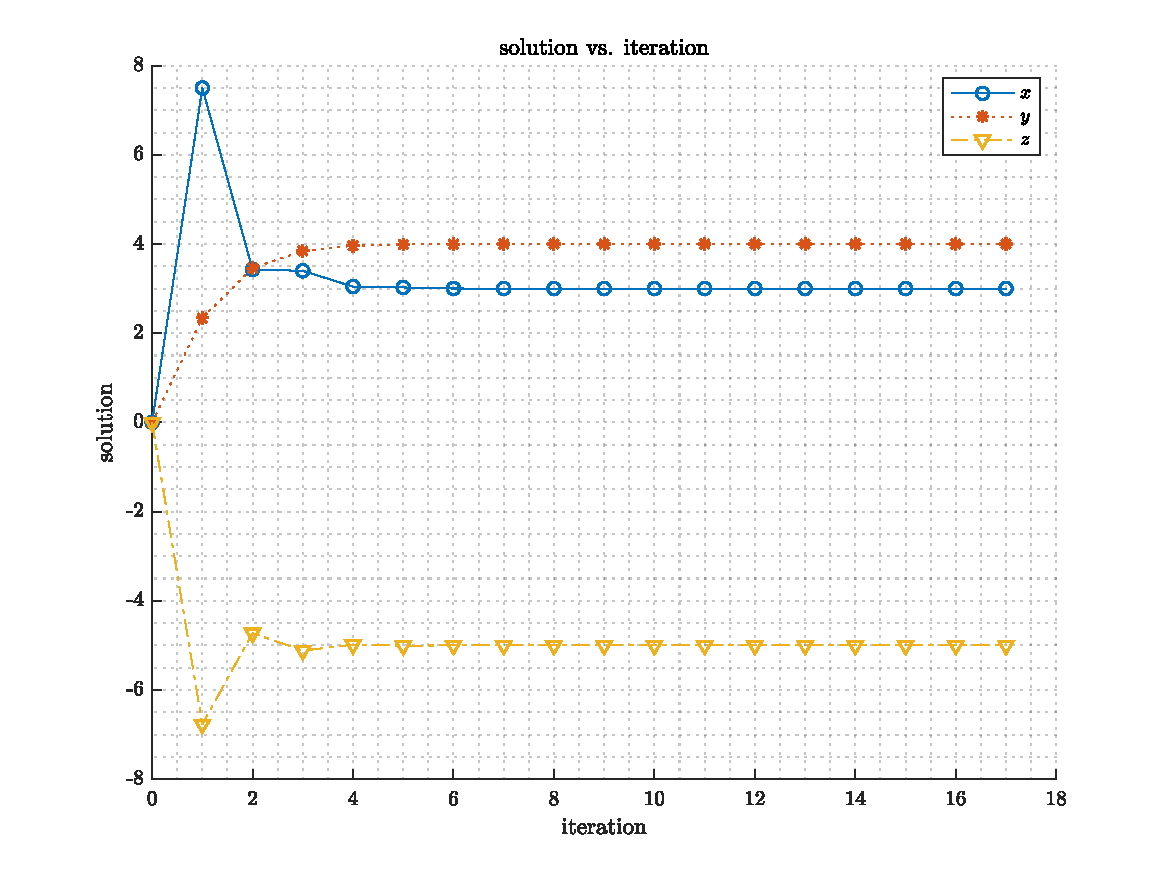
\includegraphics[width=0.80\textwidth]{../src/lab_07_plot_1.pdf}
    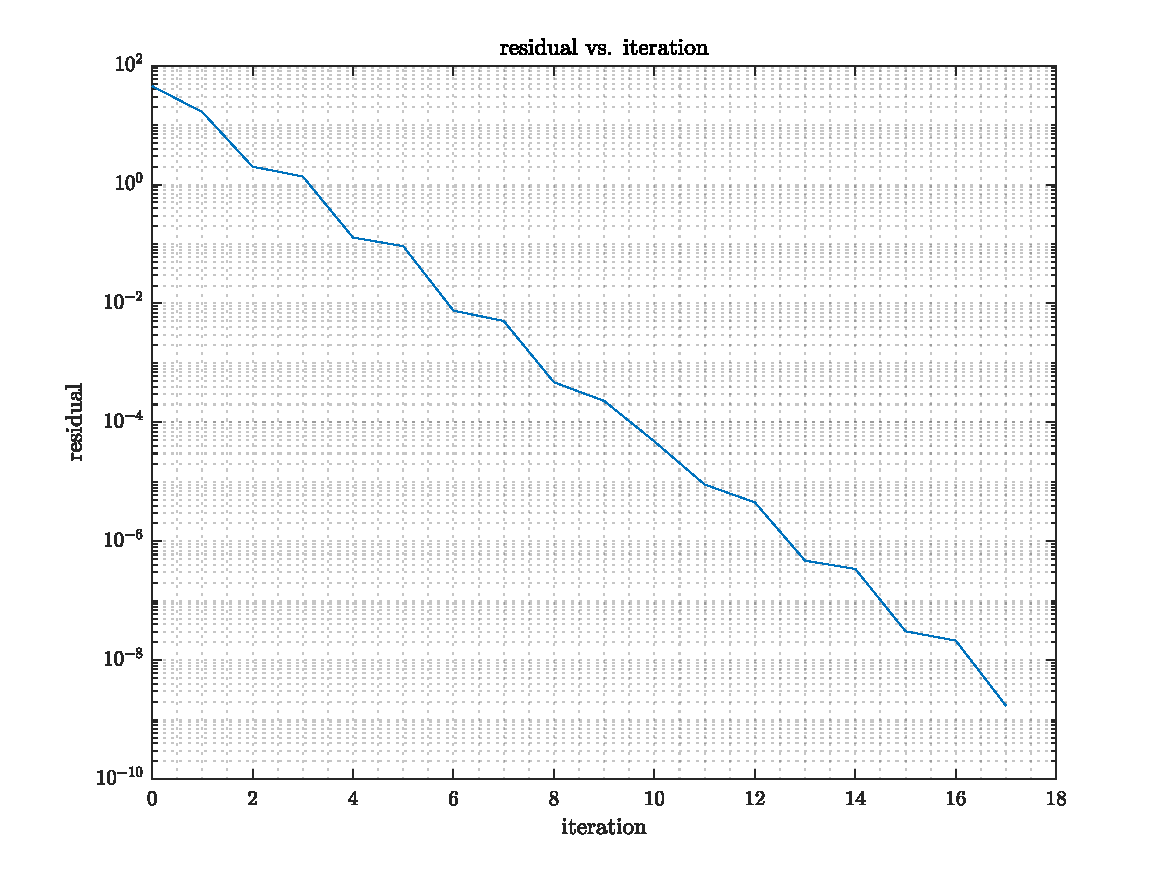
\includegraphics[width=0.80\textwidth]{../src/lab_07_plot_2.pdf}
    \caption{Solution and residual}
    \label{fig:sol}
\end{figure}
\end{verbatim}


\end{document}
| to include the table you got from MATLAB.
\end{itemize}

Recompile and submit the PDF file generated by Overleaf to WyoCourses.

\newpage
%---------------------------------------------
\section{Basics of \LaTeX{}}
\label{sec:bol}
%---------------------------------------------
\subsection{LU Decomposition}

Given the linear system \eqref{eq:varyRHS}
\begin{equation}
  \label{eq:varyRHS}
  \begin{cases}
    3x + y + z = m \\
    x - 5y + 2z = 5 \\
    2x + y + 5z = 10
  \end{cases}
\end{equation}
where $m = 0, 1, 2, \ldots, 20$. Using LU Decomposition we can obtain the solution to the linear system \eqref{eq:varyRHS} for corresponding $m$ (see Table \ref{tab:solution} and Figure \ref{fig:solution}).

%
% main.tex
%
% Copyright © 2019 Libao Jin <jinlibao@outlook.com>
% Distributed under terms of the MIT license.
%

\documentclass[11pt,oneside,letter,twoside,usename,dvipsnames,svgnames,table]{article}

% Load packages
\usepackage{
  afterpage,amsfonts,amsmath,amssymb,amsthm,appendix,array,booktabs,breqn,
  caption,color,enumerate,enumitem,fancyhdr,float,fontspec,geometry,graphicx,grffile,
  hyperref,hyphenat,ifthen,imakeidx,indentfirst,lastpage,lipsum,listings,
  longtable,makeidx,mathtools,multicol,subcaption,tikz,tikzscale,titlesec,
  titling,verbatim,xcolor,xltxtra,xunicode
}

\title{MATH 3340 - Scientific Computing Homework 8}
\author{Libao Jin}

\makeatletter
\let\Author\@author
\let\Title\@title
\makeatother
% ------------------- define \Xint ----------------
\def\Xint#1{\mathchoice
  {\XXint\displaystyle\textstyle{#1}}%
  {\XXint\textstyle\scriptstyle{#1}}%
  {\XXint\scriptstyle\scriptscriptstyle{#1}}%
  {\XXint\scriptscriptstyle\scriptscriptstyle{#1}}%
\!\int}
\def\XXint#1#2#3{{\setbox0=\hbox{$#1{#2#3}{\int}$ }
\vcenter{\hbox{$#2#3$ }}\kern-.6\wd0}}
\def\ddashint{\Xint=}
\def\dashint{\Xint-}
% ------------------- setlength -------------------
\setlength{\parindent}{0pt}
\setlength{\parskip}{5pt}
% ------------------- algorithm2e -----------------
\usepackage[ruled]{algorithm2e}
% ------------------- amsthms ---------------------
\theoremstyle{definition}
\newtheorem{definition}{Definition}[section]
\newtheorem{lemma}{Lemma}[section]
\newtheorem{corollary}{Corollary}[section]
\newtheorem{remark}{Remark}[section]
\newtheorem{claim}{Claim}[section]
\newtheorem{theorem}{Theorem}[section]
\newtheorem{example}{Example}[section]
\newtheorem{exercise}{Exercise}[section]
\newtheorem{proposition}{Proposition}[section]
\newtheorem{proc}{Procedure}[section]
\numberwithin{equation}{section}
% ------------------- define macros ---------------
\newcommand{\tightlist}{}
\newcommand{\semester}{\ifthenelse{\month<9}{\ifthenelse{\month<5}{Spring}{Summer}}{Fall} \the\year}
\newcommand{\AxisRotator}[1][rotate=0]{%
  \tikz [x=0.25cm,y=0.60cm,line width=.2ex,-stealth,#1] \draw (0,0) arc (-150:150:1 and 1);%
}
% \newcommand{\problem}{0}
\newcommand{\sol}{0}
\newcommand{\homework}{0}
\ifdefined\problem
  \newenvironment{solution}{\comment}{\endcomment}
\else
  \newenvironment{solution}{\begin{proof}[{\rm\bf Solution}]}{\end{proof}}
  \newcommand{\sectionbreak}{\clearpage}
\fi
% ------------------- titlesec --------------------
\ifdefined\homework
  \titleformat{\section}[runin]{\bf}{}{0em}{}[.]
\fi
%\titleformat{\section}{\scshape\Large}{\thesection}{1em}{}
%\titleformat{\subsection}{\scshape\large}{\thesubsection}{1em}{}
%\titleformat{\subsubsection}{\large}{\thesubsubsection}{1em}{}
%\renewcommand{\thesection}{\Roman{section}}
% ------------------- caption ---------------------
\captionsetup{width=0.95\textwidth}
% ------------------- enumitem --------------------
\setlist{noitemsep}
% \setenumerate{label=(\alph*)}
% ------------------- fontspec --------------------
% \defaultfontfeatures{Mapping=tex-text,Scale=MatchLowercase,Numbers=OldStyle}
% \setromanfont{Palatino}
% \setsansfont{Helvetica}
\setmonofont[Scale=MatchLowercase]{Monaco}
% ------------------- geometry --------------------
\geometry{
  margin = 1in
}
% ------------------- hyperref --------------------
\hypersetup{
  %--------------- pdfinfo ------------------
  pdftitle  = {\Title},
  pdfauthor = {\Author},
  pdfsubject= {\Title},
  pdfkeywords={},
  %--------------- links --------------------
  colorlinks= {true},
  linkcolor = {red},
  citecolor = {cyan},
  bookmarks = {false},
  bookmarksnumbered = {true},
  %--------------- pagemode -----------------
  pdffitwindow={true},
  pdftoolbar= {false},
  pdfmenubar= {false},
  pdfpagelayout = {OneColumn},
  pdfstartview = {FitH},
  pdfpagemode = {UseNone},
  %pdfnonfullscreenpagemode = {UseNone}
}
%------------------- fancyhdr ---------------------
\fancypagestyle{exercise-style}{
  \fancyhf{}
  \fancyhead[LO,RE]{\footnotesize \semester}
  \fancyhead[CO,CE]{\footnotesize \Title}
  \fancyhead[LE,RO]{\footnotesize\thepage\ of \pageref*{LastPage}}
  \pagenumbering{arabic}
}
\fancypagestyle{report-style}{
  \fancyhf{}
  \fancyhead[LO,RE]{\footnotesize \Author}
  \fancyhead[CO,CE]{\footnotesize \Title}
  \fancyhead[LE,RO]{\footnotesize\thepage\ of \pageref*{LastPage}}
  \pagenumbering{arabic}
}
\renewcommand{\sectionmark}[1]{\markboth{#1}{}}
\renewcommand{\subsectionmark}[1]{\markright{\thesubsection \ #1}}
\pagestyle{report-style}
% ------------------- maketitle -------------------
\makeatletter
\def\@maketitle{%
  \begin{center}%
    \let \footnote \thanks
    %{\bfseries\huge \course\ --- \semester \par \vskip .5em {\LARGE \@title}}
    {\LARGE \@title \par}
    {\vskip 1.5em \large \@author}
    {\vskip .5em \large \@date}
  \end{center}
\par \vskip .5em}
\makeatother
% ------------------- table alignment -------------
\newcolumntype{L}[1]{>{\raggedright\arraybackslash}p{#1}}
\newcolumntype{C}[1]{>{\centering\arraybackslash}p{#1}}
\newcolumntype{R}[1]{>{\raggedleft\arraybackslash}p{#1}}
% \allowdisplaybreaks
% ------------------ lstlisting ------------------
\lstset{
  basicstyle={\ttfamily\footnotesize},
  breaklines=true,
  keywordstyle=\color{Red},
  otherkeywords={},
  morekeywords={},
  identifierstyle=\color{darkgray},
  stringstyle=\color{LightCoral},
  commentstyle=\color{gray},
  showstringspaces=false,
  numberstyle={\footnotesize \color{Black}},
  numbersep=9pt,
  numbers=left,
  emph={int,char,double,float,unsigned,auto},
  emphstyle={\color{Cerulean}},
  frame=single,
  backgroundcolor=\color{White},
  tabsize=4,
  language={},
}

% Define language diff (using git diff highlighting)
\newcommand{\lstbg}[3][0pt]{{\fboxsep#1\colorbox{#2}{\strut #3}}}
\lstdefinelanguage{diff}{
  basicstyle={\ttfamily\small},
  breaklines=true,
  morecomment=[f][\lstbg{red!20}]-,
  morecomment=[f][\lstbg{green!20}]+,
  morecomment=[f][\color{blue}]{@@},
}

% Define language Golang
\lstdefinelanguage{Golang}%
{morekeywords=[1]{package,import,func,type,struct,return,defer,panic,%
  recover,select,var,const,iota,},%
  morekeywords=[2]{string,uint,uint8,uint16,uint32,uint64,int,int8,int16,%
    int32,int64,bool,float32,float64,complex64,complex128,byte,rune,uintptr,%
  error,interface},%
  morekeywords=[3]{map,slice,make,new,nil,len,cap,copy,close,true,false,%
  delete,append,real,imag,complex,chan,},%
  morekeywords=[4]{for,break,continue,range,goto,switch,case,fallthrough,if,%
  else,default,},%
  morekeywords=[5]{Println,Printf,Error,Print,},%
  sensitive=true,%
  morecomment=[l]{//},%
  morecomment=[s]{/*}{*/},%
  morestring=[b]',%
  morestring=[b]",%
  morestring=[s]{`}{`},%
}

% Define various styles for different lanuages
\lstdefinestyle{Makefile}{
  basicstyle=\ttfamily,
  breaklines=true,
  keywordstyle=\color{Red},
  otherkeywords={},
  morekeywords={},
  identifierstyle=\color{darkgray},
  stringstyle=\color{darkgray},
  commentstyle=\color{gray},
  showstringspaces=false,
  numberstyle={\footnotesize \color{Black}},
  numbersep=9pt,
  numbers=left,
  emph={int,char,double,float,unsigned,auto},
  emphstyle={\color{Cerulean}},
  frame=single,
  backgroundcolor=\color{White},
  tabsize=4,
  language=make,
}

\lstdefinestyle{MATLAB}{
  basicstyle={\ttfamily\small},
  breaklines=true,
  keywordstyle=\color{Red},
  otherkeywords={},
  alsoletter={...},
  morekeywords={break,case,catch,continue,elseif,else,end,for,function,global,
    if,otherwise,persistent,return,switch,try,while,methods,properties,
  events,classdef,...},
  comment=[l]\%,                              % comments
  morecomment=[l]...,                         % comments
  morecomment=[s]{\%\{}{\%\}},                % block comments
  morestring=[m]
  identifierstyle=\color{darkgray},
  stringstyle=\color{LightCoral},
  commentstyle=\color{gray},
  showstringspaces=false,
  numberstyle={\footnotesize \color{Black}},
  numbersep=9pt,
  numbers=left,
  emph={int,char,double,float,unsigned,auto},
  emphstyle={\color{Cerulean}},
  frame=single,
  backgroundcolor=\color{White},
  tabsize=4,
  language=MATLAB,
}

\lstdefinestyle{C++}{
  basicstyle=\ttfamily,
  breaklines=true,
  keywordstyle=\color{Red},
  otherkeywords={memset},
  morekeywords={>,<,.,;,-,!,=,~},
  identifierstyle=\color{darkgray},
  stringstyle=\color{LightCoral},
  commentstyle=\color{gray},
  showstringspaces=false,
  numberstyle={\footnotesize \color{Black}},
  numbersep=9pt,
  numbers=left,
  emph={bool,int,char,double,float,unsigned,auto,string,pair,unordered_set,vector},
  emphstyle={\color{Cerulean}},
  frame=single,
  backgroundcolor=\color{White},
  tabsize=4,
  language=C++,
}

\lstdefinestyle{Plain}{
  basicstyle={\ttfamily\footnotesize},
  breaklines=true,
  keywordstyle=\color{Red},
  otherkeywords={},
  morekeywords={},
  identifierstyle=\color{darkgray},
  stringstyle=\color{LightCoral},
  commentstyle=\color{gray},
  showstringspaces=false,
  numberstyle={\footnotesize \color{Black}},
  numbersep=9pt,
  numbers=left,
  emph={int,char,double,float,unsigned,auto},
  emphstyle={\color{Cerulean}},
  frame=single,
  backgroundcolor=\color{White},
  tabsize=4,
  language={},
}

\lstdefinestyle{TeX}{
  basicstyle={\ttfamily\footnotesize},
  breaklines=true,
  keywordstyle=\color{Red},
  otherkeywords={},
  morekeywords={},
  identifierstyle=\color{darkgray},
  stringstyle=\color{LightCoral},
  commentstyle=\color{gray},
  showstringspaces=false,
  numberstyle={\footnotesize \color{Black}},
  numbersep=9pt,
  numbers=left,
  emph={int,char,double,float,unsigned,auto},
  emphstyle={\color{Cerulean}},
  frame=single,
  backgroundcolor=\color{White},
  tabsize=4,
  language=[LaTeX]{TeX},
}

\lstdefinestyle{C}{
  basicstyle={\ttfamily\footnotesize},
  breaklines=true,
  keywordstyle=\color{Red},
  otherkeywords={},
  morekeywords={},
  identifierstyle=\color{darkgray},
  stringstyle=\color{LightCoral},
  commentstyle=\color{gray},
  showstringspaces=false,
  numberstyle={\footnotesize \color{Black}},
  numbersep=9pt,
  numbers=left,
  emph={int,char,double,float,unsigned,auto},
  emphstyle={\color{Cerulean}},
  frame=single,
  backgroundcolor=\color{White},
  tabsize=4,
  language=C,
}

\lstdefinestyle{Python}{
  basicstyle={\ttfamily\footnotesize},
  breaklines=true,
  keywordstyle=\color{Red},
  otherkeywords={},
  morekeywords={},
  identifierstyle=\color{darkgray},
  stringstyle=\color{LightCoral},
  commentstyle=\color{gray},
  showstringspaces=false,
  numberstyle={\footnotesize \color{Black}},
  numbersep=9pt,
  numbers=left,
  emph={int,char,double,float,unsigned,auto},
  emphstyle={\color{Cerulean}},
  frame=single,
  backgroundcolor=\color{White},
  tabsize=4,
  language=Python,
}


\lstdefinestyle{Golang}{
  basicstyle={\ttfamily\footnotesize},
  breaklines=true,
  keywordstyle=\color{Red},
  otherkeywords={},
  morekeywords={},
  identifierstyle=\color{darkgray},
  stringstyle=\color{LightCoral},
  commentstyle=\color{gray},
  showstringspaces=false,
  numberstyle={\footnotesize \color{Black}},
  numbersep=9pt,
  numbers=left,
  emph={int,char,double,float,unsigned,auto},
  emphstyle={\color{Cerulean}},
  frame=single,
  backgroundcolor=\color{White},
  tabsize=4,
  language=Golang,
}

\lstdefinestyle{diff}{
  basicstyle={\ttfamily},
  breaklines=true,
  keywordstyle=\color{black},
  otherkeywords={},
  morekeywords={},
  identifierstyle=\color{black},
  stringstyle=\color{black},
  commentstyle=\color{gray},
  showstringspaces=false,
  numberstyle={\footnotesize \color{Black}},
  numbersep=9pt,
  numbers=left,
  emph={},
  emphstyle={\color{black}},
  frame=single,
  backgroundcolor=\color{White},
  tabsize=4,
  language=diff,
}

\begin{document}
% \ifx\undefined\sol
\thispagestyle{empty}
\maketitle
% \fi
\section{Output: \lstinline[style=Plain]{lab_06_output.txt}}
\lstinputlisting[style=Plain]{../src/lab_06_output.txt}
\newpage
\section{Script: \lstinline[style=Plain]{lab_06_script.m}}
\lstinputlisting[style=MATLAB]{../src/lab_06_script.m}
\newpage
\section{Basics of \LaTeX{}}
% PUT YOUR REPRODUCING CODE HERE
\begin{verbatim}
\subsection{Output}

\lstinputlisting[style=Plain]{../src/lab_07_output.txt}

\subsection{Formatted output}

\input{../src/sor_gauss_seidel.tex}

\newpage

\subsection{Plots}
\begin{figure}[!hbtp]
    \centering
    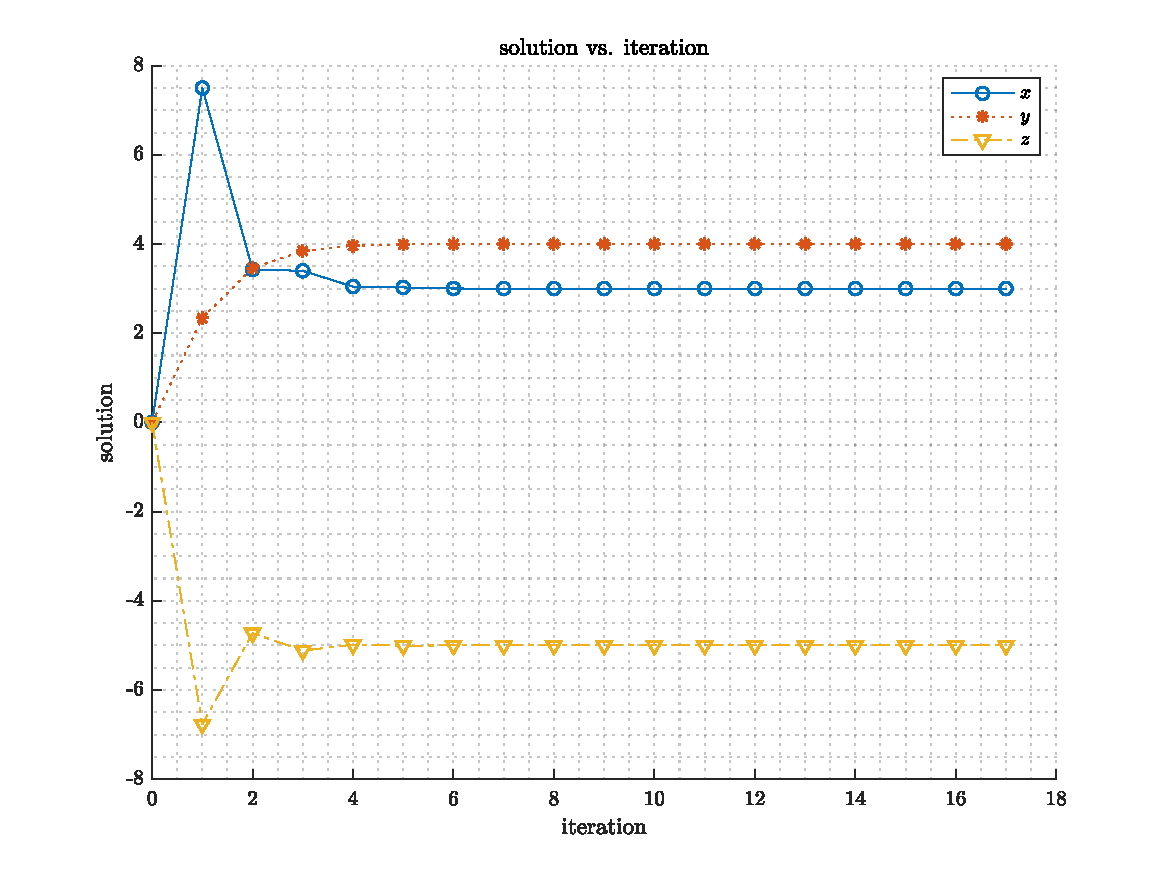
\includegraphics[width=0.80\textwidth]{../src/lab_07_plot_1.pdf}
    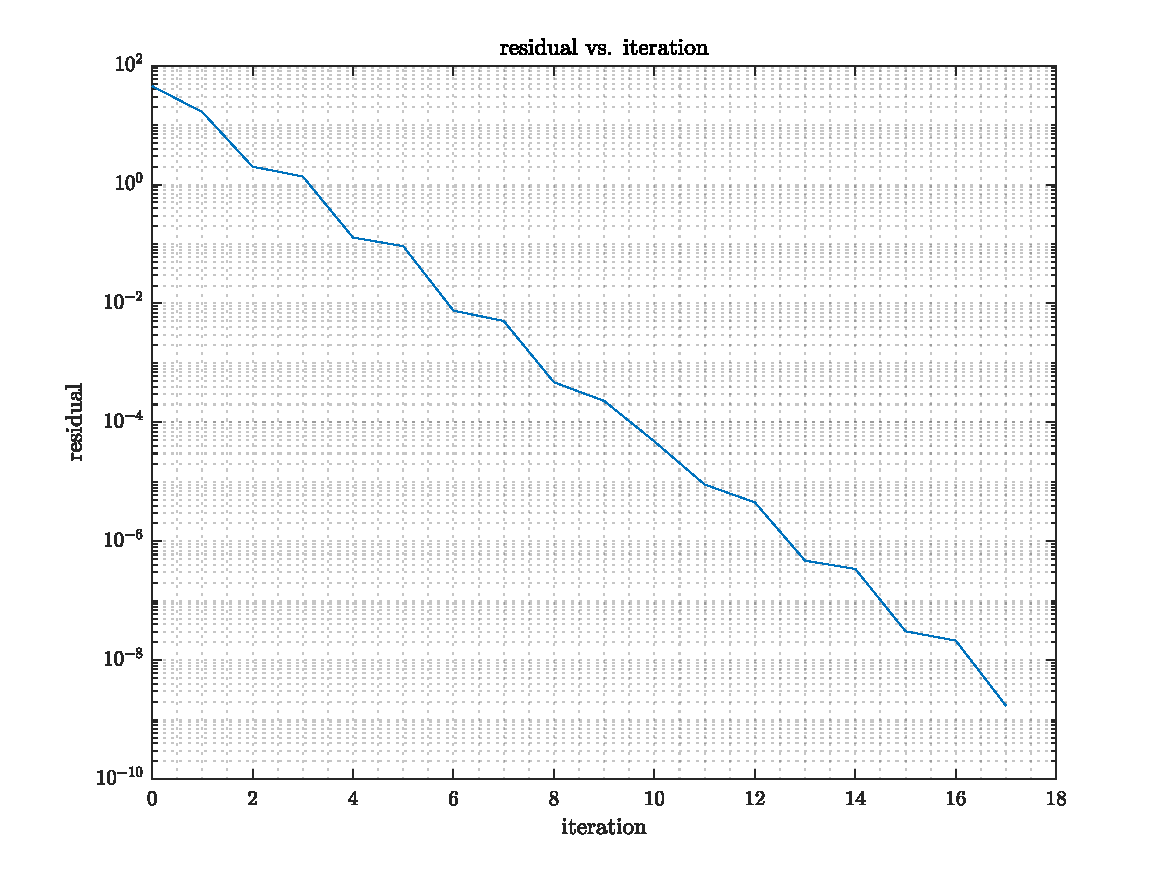
\includegraphics[width=0.80\textwidth]{../src/lab_07_plot_2.pdf}
    \caption{Solution and residual}
    \label{fig:sol}
\end{figure}
\end{verbatim}


\end{document}


\begin{figure}[!hbtp]
  \centering
  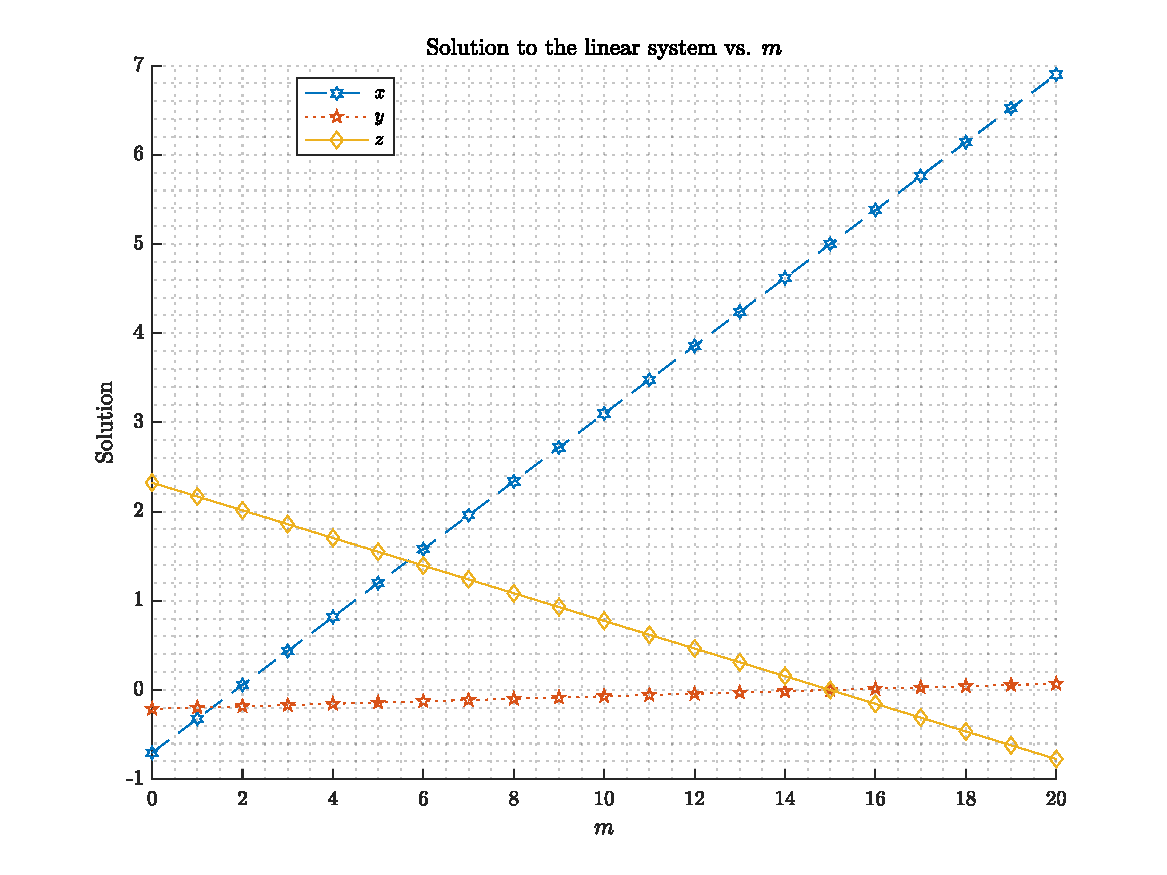
\includegraphics[width=0.85\textwidth]{../Math.3341.Lab.06.ans/lab_06_plot.pdf}
  \caption{Solution to the linear system vs. $m$}
  \label{fig:solution}
\end{figure}
